\documentclass[10pt,landscape,a4paper]{article}

% Import settings
%! PACKAGES

\usepackage[margin=1cm,landscape]{geometry}
\geometry{
  a4paper,
  left=10mm,
  right=10mm,
  headheight=1cm,
  top=1cm,
  bottom=1.5cm,
  footskip=1cm,
  %showframe
}

%\usepackage{lipsum}

\usepackage{hyperref} % For hyperlinks
\hypersetup{
    colorlinks=true,
    %linkcolor=blue,
    %filecolor=magenta,
    urlcolor=cyan,
}

\usepackage{multicol} % For overall column layout
\usepackage{xcolor} % For colors
\usepackage{tabularx}
\usepackage{fancyhdr} % For footer
\usepackage{multirow}   % multirow



\pagenumbering{gobble} % No page numbering
\pagestyle{fancy}
\fancyhead{} % No header
\renewcommand{\headrulewidth}{0pt} % No header rule

\cfoot{\copyright~2019 Canonical} % Actual footer text

% A bunch of command for boilerplate text
\newcommand{\clicmd}[1]{\textbf{\sffamily\color{blue}#1}~~}
\newcommand{\cliverb}[1]{{\sffamily\color{blue}#1}~~}
\newcommand{\cliopt}[1]{{\sffamily#1}~~}
\newcommand{\textangles}[1]{\textless #1\textgreater}
\newcommand{\smallhspace}{\-\hspace{0.3cm}}
\newcommand{\terminal}[1]{\-\hspace{0.2cm}{\sffamily\$ #1}}
\newcommand{\terminalinebreak}[1]{\ \textbackslash\hfill\phantom{.}\linebreak\-\hspace{0.5cm}~}
\newcommand{\ddash}{-{}-}
\newcommand{\deprecated}[1]{{\color{orange}(deprecated)#1}}





\title{Python Cheatsheed}
\author{}
\date{}



%%%%%%%%%%%%%%%%%%%%%%%%%%%%%%%%%%%%%%%%%%%%%%%%%% 
%%%%%%%%%%%%%%%%%%%% Document %%%%%%%%%%%%%%%%%%%%
%%%%%%%%%%%%%%%%%%%%%%%%%%%%%%%%%%%%%%%%%%%%%%%%%% 


\begin{document}

    \maketitle
    \footnotesize           % small text

    % Table of contents
    \begin{multicols}{3}
        \tableofcontents
    \end{multicols}
    \newpage



    %%%%%%%%%%%%%%%%%% Foundamentals %%%%%%%%%%%%%%%%%% 
    \section{Foundamentals}
        \begin{multicols}{3}
            \subsection{Data types}

\begin{tabularx}{\linewidth}{@{}| l | l | X |@{}}
    \hline
    Name & Data type & Description \\
    \hline
    string & 'str' & sequence of characters \\ 
    integer & 1 & integers numbers \\
    float & 0.1 & decimals numbers \\
    complex & 1j & imaginary numbers \\
    boolean & True/False & logical values \\
    list & [a, b, ...] & mutable ordered sequence \\
    tuple & (a, b, ...) & immutable ordered sequence \\
    range & range(init, fin, step) & immutable ordered sequence \\
    dictionary & \{key=value, ...\} & mutable unordered mapping \\
    set & \{x, ...\} &  mutable unordered set \\
    frozenset & frozenset(\{x, ...\}) & immutable unordered set \\
    byte & & \\
    bytearray & & \\
    memoryview & & \\
    \hline
\end{tabularx}



\subsubsection{Data conversion}

\begin{tabular}{@{}ll@{}}
    \verb!!    & convert in string data type \\
    \verb!int()!    & convert in integer data type \\
    \verb!float()!    & convert in float data type \\
    \verb!bool()!    & convert in bool data type \\
    \verb!list()!    & convert in list data type \\
    \verb!dict()!    & convert in dict data type \\
    \verb!set()!    & convert in set data type \\
\end{tabular}



\subsubsection{Generic operations}
\begin{tabular}{@{}ll@{}}
    \verb!len(x)!    & variable length \\
    \verb!min(x), max(x)!    & min/max value \\
    \verb!sorted(x)!    & sort a list \\
    \verb!enumerate(x, ...)!    & iterator \\
    \verb!zip(x)!    & iterator on tuple \\
    \verb!all(x)!    & true if all are true \\
    \verb!any(x)!    & true if at least one is true \\
\end{tabular}


\subsubsection{Sting operations}
\begin{tabular}{@{}ll@{}}
    \verb!s1 + s2!    & concatenation \\
    \verb!s * int!    & multiplication \\
    \verb!s[i]!    & indexing \\
    \verb!s.index()!    & ?? \\
    \verb!s.find()!    & ?? \\
    \verb!s.strip()!    & remove white spaces \\
    \verb!s.lower()!    & lowercase \\
    \verb!s.upper()!    & uppercase \\
    \verb!s.split([sep])!    & creates string array of words \\
    \verb!s.join(seq)!    & creates string array of words \\
    \verb!s.find('string')!    & match string in string \\
    \verb!s.replace('old', 'new')!    & replace string \\
\end{tabular}


\subsubsection{List operations}
\begin{tabular}{@{}ll@{}}
    \verb!l.append(x)!    & append a element \\
    \verb!l.extend(x)!    & append as sequence of elements \\
    \verb!l.insert(i,x)!    & insert variable at i position \\
    \verb!l.remove(x)!    & remove value x \\
    \verb!l.pop([i])!    & remove and return item at index i \\
    \verb!l.sort()!    & sort \\
    \verb!l.revert()!    & reverse sort \\
\end{tabular}


\subsubsection{Dictionaries operations}
\begin{tabular}{@{}ll@{}}
    \verb!d[key] = value!    & assign value to a key \\
    \verb!d.clear()!    & clear dictionary \\
    \verb!d.update(d2)!    & ?? \\
    \verb!d.key()!    & ?? \\
    \verb!d.values()!    & ?? \\
    \verb!d.items()!    & ?? \\
    \verb!d.pop(key[default])!    & ?? \\
    \verb!d.popitem()!    & ?? \\
    \verb!d.get(key[default])!    & ?? \\
    \verb!d.setdefault(key[default])!    & ?? \\
\end{tabular}


\subsubsection{Sets operations}
\begin{tabular}{@{}ll@{}}
    \verb!s.update(s2)!    & ?? \\
    \verb!s.copy()!    & ?? \\
    \verb!s.add(key)!    & ?? \\
    \verb!s.remove(key)!    & ?? \\
    \verb!s.discard(key)!    & ?? \\
    \verb!s.clear()!    & ?? \\
    \verb!s.pop()!    & ?? \\
\end{tabular}






\section{Operators}

    \subsection{Arithmetic operators}
        \begin{tabular}{@{}ll@{}}
            \verb!+, -, *, /!    & basic operations \\
            \verb!%!     & module \\
            \verb!**!      & exponential \\
            \verb!//!      & floor \\
        \end{tabular}
        
    \subsection{Logic operators}
        \begin{tabular}{@{}ll@{}}
            \verb!==!    & equal \\
            !=    & not equal \\
            \verb!<,>!     & strict inequality \\
            \verb!<=,>=!      & inequality \\
        \end{tabular}


    \subsection{Boolean operators}
        \begin{tabular}{@{}ll@{}}
            \verb!x and y!    & and operator \\
            \verb!x or y!    & or operator \\
            \verb!not x!    & not operator \\
        \end{tabular}
        
        
    \subsection{Assignment operators}
        \begin{tabular}{@{}ll@{}}
            \verb!=!    & value assignment \\
            \verb!+=, -=, *=, /=, **=, //=!    & arithmetic assignment \\
            % \verb!&=, \|=!    & logic assignment \\
            % \verb!^=!    & ?? \\
            % \verb!>>=, <<=!    & ?? \\
        \end{tabular}
        
        
    \subsection{Other operators}
        \begin{tabular}{@{}ll@{}}
            \verb!x is y!    & true if x is y \\
            \verb!x is not y!    & true if x is not y \\
            \verb!x in y!    & true x is in y sequence \\
            \verb!x not in y!    & true x is not in y sequence \\
        \end{tabular}
        
        
    \subsection{Indexing}
        \begin{tabular}{@{}ll@{}}
            \verb!x[i]!    & list i-th element \\
            \verb!x[init_val:fin_val]!    & list slicing \\
        \end{tabular}







\subsection{Loops/Conditions}

\subsubsection{if/elif/else}

\begin{minted}{python}
if condition:
    ...
elif condition:
    ...
else:
    default
\end{minted}


\subsubsection{while}

\begin{minted}{python}
while condition:
    ...
\end{minted}


\subsubsection{for}

\begin{minted}{python}
\for condition:
    ...
\end{minted}


Keywords:
\begin{tabular}{@{}ll@{}}
    \verb!break!    & end the loop \\
    \verb!continue!    & continue the loop \\
    \verb!\t!    & tab \\
\end{tabular}


    


\subsection{Functions}

\begin{minted}{python}
# function definition
def fun_name(param, *args, param=default, **kwargs):
    # function body
    ...
    return x    # value to return

# function call
a = fun_name(arg_1, ..., arg_n))
\end{minted}





\subsection{Input/Output}

\begin{tabular}{@{}ll@{}}
    \verb!print(x)!    & print function \\
    \verb!x = input("string: ")!    & input function \\
\end{tabular}

Keywords:
\begin{tabular}{@{}ll@{}}
    \verb!\n!    & newline \\
    \verb!\s!    & space \\
    \verb!\t!    & tab \\
\end{tabular}










\subsection{Filesystem}

\begin{tabular}{@{}ll@{}}
    \verb!f = open("file","mode",encoding="enc")!    & open file \\
    \verb!f.write(text)!    & writing \\
    \verb!f.writelines(list of lines)!    & writing \\
    \verb!f.read()!    & reading chars \\
    \verb!f.readlines()!    & reading lines \\
    \verb!f.readline()!    & next line \\
    \verb!f.close()!    & close file \\
\end{tabular}\\
mode: \\
- r: read \\
- a: append \\
- w: write \\
- x: create \\
enc: \\
- utf8 \\
- ascii \\
- latin1 \\


\begin{minted}{python}
# open file
with open("file", "mode") as f:
    for line in f:
        ...
\end{minted}







\subsection{Error Handling}

\begin{minted}{python}
raise ExcClass()
try:
    <code>
except Exception as exc:
    <error>
\end{minted}





        \end{multicols}
    \newpage


    %%%%%%%%%%%%%%%%%% Common Modules %%%%%%%%%%%%%%%%%% 
    \section{Common Modules}
        \begin{multicols}{3}
            \subsection{Math}

\begin{minted}[breaklines=true]{python}
import math
\end{minted}

\begin{tabular}{@{}ll@{}}
    \verb!!    & absolute value \\
    \verb!!    & round value \\
    \verb!()!    & sine \\
    \verb!cos()!    & cosine \\
    \verb!tan()!    & tangent \\
    \verb!sqrt()!    & square root \\
    \verb!log()!    & logarithm \\
    \verb!ceil()!    & ceil \\
    \verb!floor()!    & floor \\
\end{tabular}



\subsection{Argumens Parser}

\begin{minted}[breaklines=true]{python}
import argparse

# create object
arg = argparse.ArgumentParser()

# add argument
arg.add_argument('-strink_arg_name', 'full_arg_name', required=True, help='description')

args = vars(arg.parse_args())
\end{minted}



\subsection{Filesystem}

\begin{minted}[breaklines=true]{python}
from pathlib import Path

# creating path
address = Path('home', '...', 'file')
actual_path = Path.cwd()
home_path = Path.home()

# absolute path
address.is_absolute()

# get path parts
address.parent      # previous folder
address.name        # final position
address.stem        # home
address.drive
\end{minted}



\subsection{File Management}

\subsubsection{csv}

\begin{minted}[breaklines=true]{python}
import csv

# write
f = open('file.csv', 'w', newline = '')
f_csv = csv.writer(f, delimiter='\t', lineterminator='\n\n')
f_csv.writerow(['elem_0', ..., 'elem_n'])

# write as dictionary
f = open('file.csv', 'w', newline = '')
f_csv = csv.DictWriter(f, ['key_0', ..., 'key_n'])
f_csv.writeheader()
f_csv.writerow({'key_0': value_0, ..., 'key_n': value_n})

# read
f = open('file.csv', 'r')
f_csv = csv.reader(f)
for row in f_csv:
    print('Row #' + str(f_csv.line_num) + ' ' + str(row))

# read dictionary
f = open('file.csv')

f_csv = csv.DictReader(f, ['key_0', ..., 'key_n'])
for row in f_csv:
    print(row['key_0'], ..., row['key_n'])

# close
f.close()
\end{minted}


\subsubsection{json}

\begin{minted}[breaklines=true]{python}
import json

# write
json_write = {'key_0': value_0, ..., 'key_n': value_n}
stringOfJsonData = json.dumps(json_write)

# read
json_read = '{'key_0': value_0, ..., 'key_n': value_n}'
jsonDataAsPythonValue = json.loads(json_read)
print(jsonDataAsPythonValue)
\end{minted}



\subsection{Regular Expression}

\begin{minted}[breaklines=true]{python}
# object
regex_obj = re.compile(r'string_to_match')

# find the first result
match = regex_obj.search(Text)
regex_obj.search.group()
regex_obj.search.groups()

# find all results and replace
match = regex_obj.findall(Text)

# censoring data
Censored_Text = regex_obj.sub(r'CENSORED', Text)
\end{minted}


\begin{tabular}{@{}ll@{}}
    string\_to\_match: \\
    \verb!string!    & specific string \\
    \verb!(\d\D{1})(\w{2}\W)!    &  \\
    \verb!(...)!    & grouping \\
    \verb![]!    & create a character class \\
    \verb!+!    & match one or more characters \\
    \verb!*!    & match zero or more characters \\
    \verb!?!    & match zero or one character \\
    \verb!.!    & match any character except for newline \\
    \verb!^string!    & start with \\
    \verb!string&!    & end with \\
\end{tabular}








\subsection{Green thread process}
Multi-threading (aka "Green thread process") is used in IO applications.

\begin{minted}[breaklines=true]{python}
import threading

def fun_name(...):
    ...

# thread 1
t1 = threading.Thread(target=fun_name)
t1.deamon = True
t1.start()

# thread 2
t2 = threading.Thread(target=fun_name)
t2.deamon = True
t2.start()
\end{minted}
        

        


\subsection{Multiprocessing}
This method is the proper multi-threading.

\begin{minted}[breaklines=true]{python}
import numpy as np
from numba import njit
from concurrent.futures import ThreadPoolExecutor

# function definition
def fun_name(...):
    ...

# multi-process function
multi_fun = njit(fun_name, nogil=True)


# process 1
with ThreadPoolExecutor(8) as ex:
    ex.map(multi_fun, range(100))

# process 2
with ThreadPoolExecutor(8) as ex:
    ex.map(multi_fun, range(10))
\end{minted}




        \end{multicols}
    \newpage


    %%%%%%%%%%%%%%%%%% Modules Management %%%%%%%%%%%%%%%%%% 
    \section{Modules Management}
        \begin{multicols}{3}
            %%%%%%%%%%%%%%%%%% Management %%%%%%%%%%%%%%%%%% 

\section{Virtual Environment}

    \begin{tabular}{@{}ll@{}}
        \verb!python3 -m venv ws_name!    & create virtual environment \\
        \verb!source ws_name/bin/activate!    & activate virtual environment \\
        \verb!deactivate!    & deactivate virtual environment \\
    \end{tabular} \\
        


\section{Package Installer}

    \subsection{Basic commands}

        \begin{tabular}{@{}ll@{}}
            \verb!pip3 list!    & list of installed packages \\
            \verb!pip3 install!    & install packages \\
            \verb!pip3 unistall!    & unistall packages \\
            \verb!pip3 show!    & info about package \\
            \verb!pip3 check!    & verify dependencies \\
            \verb!pip3 search!    & search PyPI for packages \\
        \end{tabular} \\
    
    \subsection{Python dependancies}
    
        \begin{tabular}{@{}ll@{}}
            \verb!pip3 freeze > deps.txt!    & create list of dependencies \\
            \verb!pip3 install -r deps.txt!    & install dependencies from list \\
            \verb!pip3 uninstall -r deps.txt!    & unistall dependencies from list \\
        \end{tabular} \\


        \end{multicols} 
    \newpage


    %%%%%%%%%%%%%%%%%% Object Oriented Programming %%%%%%%%%%%%%%%%%% 
    \section{Object Oriented Programming}
        \begin{multicols}{3}
            \subsection{Introduction}

\subsubsection{Principles}

    \begin{itemize}
        \item Abstraction
        \item Encapsulation
        \item Inheritance
        \item Polimorphism
    \end{itemize}


\subsubsection{Rules}

    \begin{itemize}
        \item S
        \item O
        \item L
        \item I
        \item D
    \end{itemize}




\subsection{Class}

\begin{minted}{python}

class ClassName:

    # Constructor
    def __init__(self, args):
        self.field = value

    # Method definition
    def method(self, args):
        ...


# Child class (Inheritance)
class ChildClassName(ClassName):

    # Static attribute (class attributes definition)
    class_attribute = value

    def __init__(self, args):
        super().__init__(self, args)
        self.field = value

        # modify class attribute
        ClassName.class_attribute = value

        # call class method
        ClassName.classmethod()

    # Static method (class method definition)
    @classmethod
    def class_method(cls):
        cls.class_attribute = value

\end{minted}



        \end{multicols}
    \newpage


    %%%%%%%%%%%%%%%%%% Data Plotting %%%%%%%%%%%%%%%%%% 
    \section{Data Plotting}
        \begin{multicols}{3}
            \begin{minted}{python}
import matplotlib.pyplot as plt
\end{minted}


\subsection{Plot}

\begin{minted}{python}
fig, axes = plt.subplots(figsize=(12,6))

axes.plot(
    x, y, 
    color='value', 
    linewidth=value,
    marker='value', 
    markersize=value, 
    label='string'
)

plt.show()
\end{minted}


\subsection{Subplot}

\begin{minted}{python}
plot_obj = plt.subplots(nrows=nx, ncols=ny, figsize=(12,6))
fig, (axes_0, ..., axes_n) = plot_obj

# subplot 0
axes_0.plot(
    x0, y0, ...
)

...

# subplot n
axes_n.plot(
    xn, yn, ...
)

plt.show()
\end{minted}


\subsection{Scatter}
    
\subsection{Bar}

\subsection{Histogram}

\subsection{Kernel density estimator}


        \end{multicols}
    \newpage


    %%%%%%%%%%%%%%%%%% Data Analysis %%%%%%%%%%%%%%%%%% 
    \section{Data Analysis}
        \begin{multicols}{3}
            \section{Introduction}

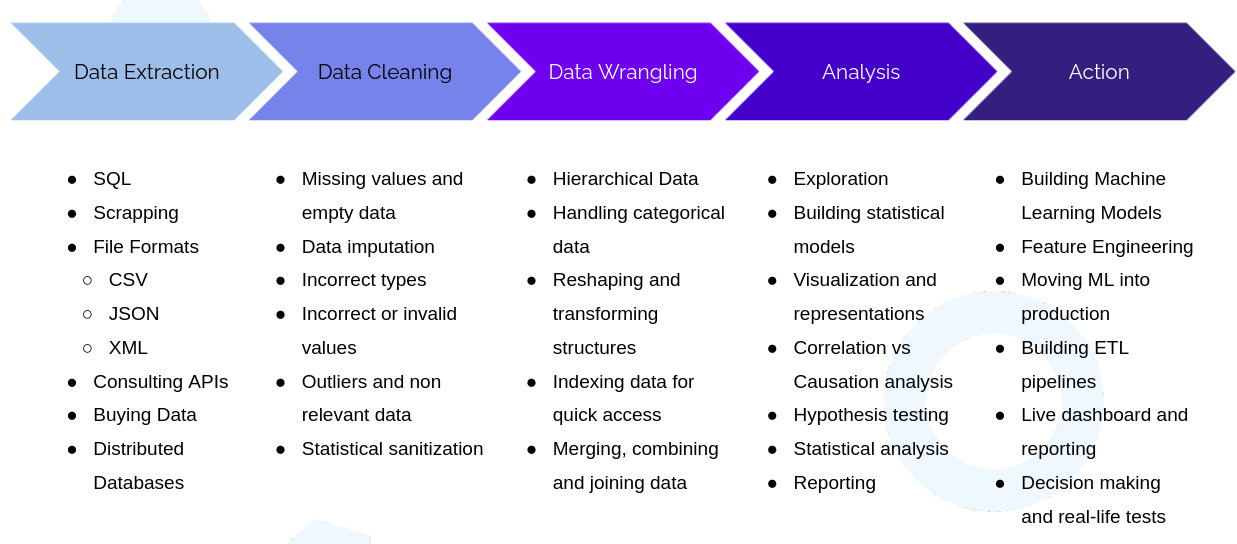
\includegraphics[scale=0.2]{pictures/data_analysis_process.png}

Useful libraries:
\begin{itemize}
  \item pandas
  \item numpy
  \item matplotlib
  \item scipy
\end{itemize}



\section{Read/Write files}

\begin{minted}{python}
    df = pd.read_csv(csv_file_name)
    df.to_csv('file_name.csv')
\end{minted}


\section{DataFrame}

\begin{minted}{python}
    # Create dataframe
    df = pd.DataFrame({
        'col_1': value.index,
        'col_2': value,
        ...
    })

    # Analysis
    df.info()           # info about dataset
    df.description()    # statistical info about dataset
    df.columns()        # dataframe columns

    # Indexing
    x = df.column_title                 # single column target
    x = df[['culumn_title_1'], ...]     # multiple columns targets

    
\end{minted}


        \end{multicols} 
    \newpage




\end{document}




% \begin{minted}{python}
% \end{minted}


% \begin{minted}[bgcolor=LightGray,framesep=1mm,baselinestretch=1,fontsize=\footnotesize,linenos=false,autogobble=true,breaklines=true,samepage=true,mathescape=true]{python}

%     # function definition
%     def fun_name(param, *args, param=default, **kwargs):
%         # function body
%         ...
%         return x    # value to return

%     # function call
%     a = fun_name(arg_1, ..., arg_n))

%     \end{minted}


% \begin{codebox}{python}{}
% class ClassName:

%     # Constructor
%     def __init__(self, args):
%         self.field = value
    
%     # Method definition
%     def method(self, args):
%         ...
% \end{codebox}